%!TEX program = xelatex
\documentclass[aspectratio=169]{ctexbeamer}

% --- 基本包 ---
\usepackage{graphicx} % 用于插入图片
\usepackage{amsmath}  % 用于数学公式
\usepackage{amssymb}  % 用于数学符号
\usepackage{booktabs} % 用于更好看的表格 (可选)
\usepackage{multirow} % 用于表格中合并单元格 (可选)

% --- USTC Beamer 主题 ---
\usepackage[bluetheme]{ustcbeamer} % 你可以选择 bluetheme, redtheme, blacktheme
\input{ustctheme.tex}
% \definecolor{themecolor}{RGB}{0,150,150} % 如果需要自定义主题颜色,取消注释并修改

% --- 文档信息 ---
\title[静电逆问题PINN]{ % 页脚的短标题
    基于物理信息神经网络的静电荷分布逆向重建研究
}
\author[金天昊]{金天昊 PB24000144} % 页脚的报告人
\institute[USTC]{
    中国科学技术大学
}
\date{2025年6月19日}

\begin{document}

%--------------------
% 标题页
%--------------------
\maketitleframe

%--------------------
% 目录页 (可选,如果内容很多)
%--------------------
\begin{frame}
    \frametitle{目录}
    \tableofcontents[hideallsubsections] %仅显示节
\end{frame}

%--------------------
% 节目录页设置 (可选,如果需要每节开始时显示)
%--------------------
\AtBeginSection[]{
\setbeamertemplate{footline}[footlineoff]%取消页脚
  \begin{frame}%
    \frametitle{目录}
    \tableofcontents[currentsection,subsectionstyle=show/show/hide]%高亮当前节
  \end{frame}
\setbeamertemplate{footline}[footlineon]%添加页脚
}

%----------------------------------------------------------------------------------
\section{研究背景与意义}
%----------------------------------------------------------------------------------
\begin{frame}
	\frametitle{研究背景与意义}
	\begin{itemize}
		\item 静电场在材料科学、半导体器件、生物电等,均有重要应用。
		\item 泊松方程 $\nabla^2\phi = -\frac{\rho}{\varepsilon_0}$,描述电荷 $\rho$ 与电势 $\phi$ 关系。
		\item \textbf{静电逆问题:} 从可观测的电势分布推断未知的电荷源,具有重要应用前景。
		\pause
		\item \textbf{应用领域:}
		\begin{itemize}
				\item \textbf{地球物理勘探:} 推断地下矿物分布、地下水探测
				\item \textbf{医学诊断:} 心电图分析、脑电图异常放电区域识别
				\item \textbf{无损检测:} 材料缺陷检测、腐蚀监测、电子器件故障诊断
		\end{itemize}
		\pause
		\item \textbf{挑战:}
		\begin{itemize}
				\item 测量数据通常稀疏且带有噪声。
				\item 传统数值微分方法对噪声敏感,直接计算 $\rho = -\varepsilon_0 \nabla^2\phi$ 结果不稳定。
		\end{itemize}
	\end{itemize}
\end{frame}


%----------------------------------------------------------------------------------
\section{研究目标与方法}
%----------------------------------------------------------------------------------
\begin{frame}
  \frametitle{研究目标}
    \begin{itemize}
        \item 利用物理信息神经网络 (PINN) 解决静电荷分布的逆向重建问题。
        \item 探究不同电荷源类型(光滑 vs. 非光滑)对 PINN 重建效果的影响。
        \item 评估测量数据质量(数据点数量、噪声水平)对重建精度的影响。
    \end{itemize}
\end{frame}
\begin{frame}
	\frametitle{研究方法:物理信息神经网络 (PINN)}
		\begin{columns}[T]
				\begin{column}{0.5\textwidth}
						\textbf{核心思想:}
						\begin{itemize}
								\item 神经网络近似未知函数 (电势 $\phi$, 电荷 $\rho$)。
								\item 损失函数包含两部分:
										\begin{itemize}
												\item \textbf{物理约束:} 偏微分方程 (泊松方程) 的残差。
												\item \textbf{数据约束:} 与已知测量点或边界条件的拟合程度。
										\end{itemize}
						\end{itemize}
				\end{column}
				\begin{column}{0.5\textwidth}
						\textbf{逆问题策略:}
						\begin{itemize}
								\item 端到端学习:同时输出电势 $\phi_{NN}$ 和电荷密度 $\rho_{NN}$。
								\item 损失函数: $L = L_{PDE}(\phi_{NN}, \rho_{NN}) + L_{BC}(\phi_{NN}) + L_{Data}(\phi_{NN}, \phi_{measured})$
						\end{itemize}
				\end{column}
		\end{columns}
		\vspace{1em}
		\begin{center}
				% 请在这里插入你的 PINN 原理图
				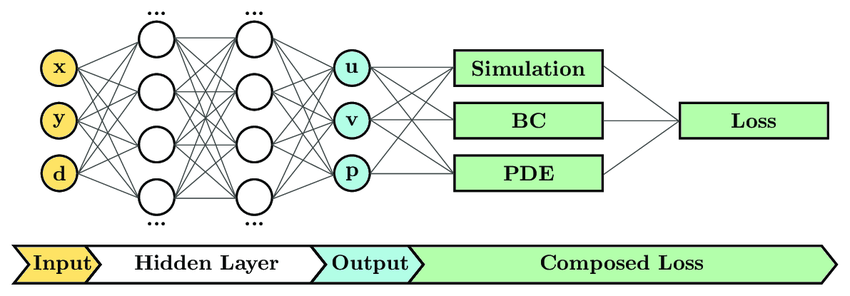
\includegraphics[width=0.5\textwidth]{figures/pinn_schematic.png}

				\small PINN 结构示意图 (示例)
		\end{center}
\end{frame}
\begin{frame}
	\frametitle{正向问题求解 (PINN能力展示)}
	\begin{columns}[T]
		\begin{column}{0.5\textwidth}
			\centering
			\textbf{方形电荷} \\
			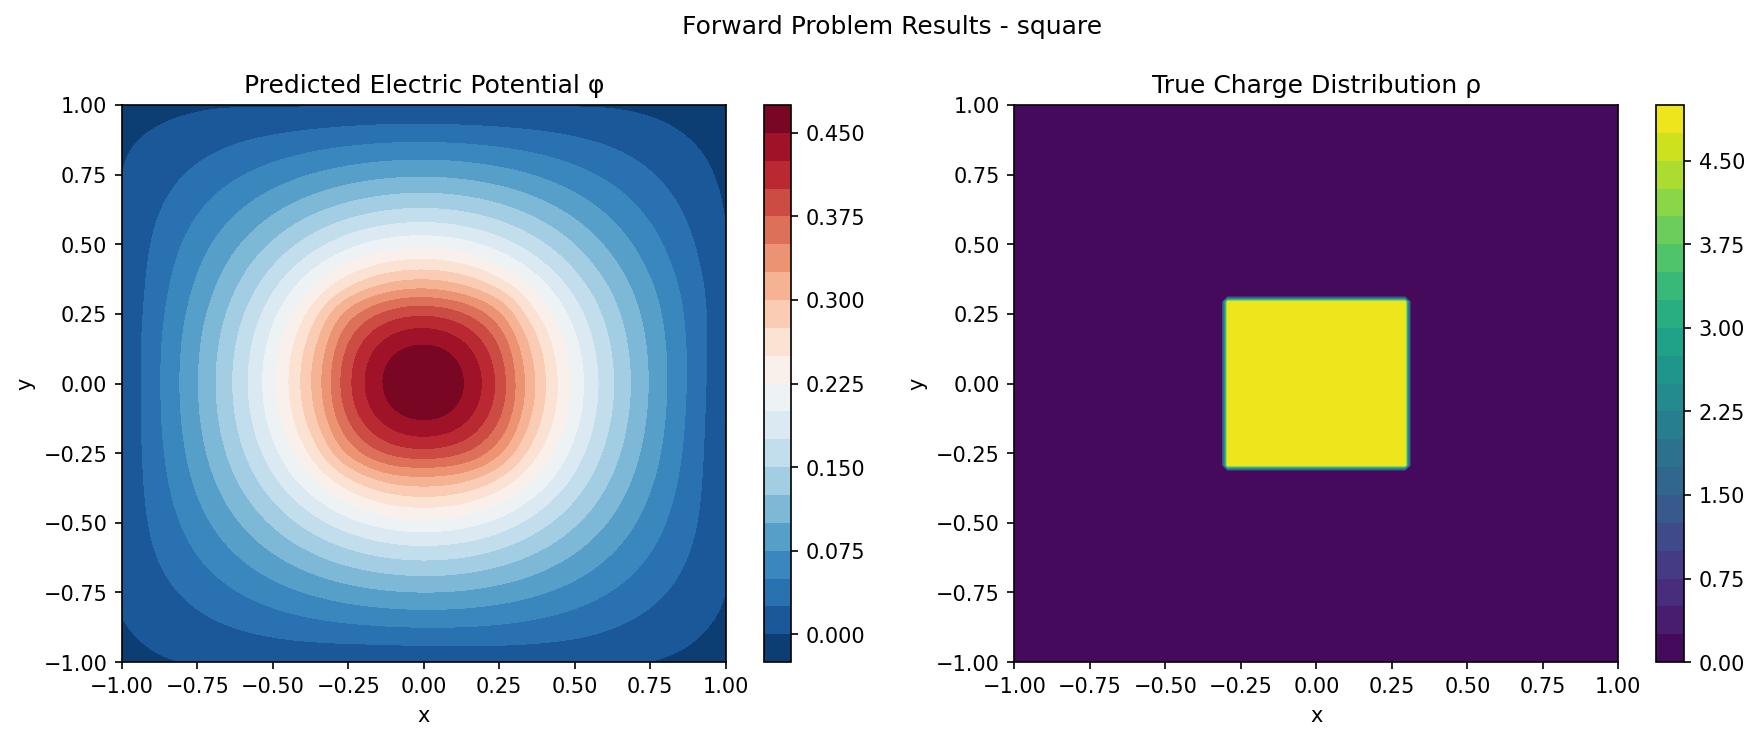
\includegraphics[width=0.9\textwidth]{figures/forward_square_combined.png} \\
			\tiny 方形电荷分布与对应电势场
		\end{column}
		\begin{column}{0.5\textwidth}
			\centering
			\textbf{高斯电荷} \\
			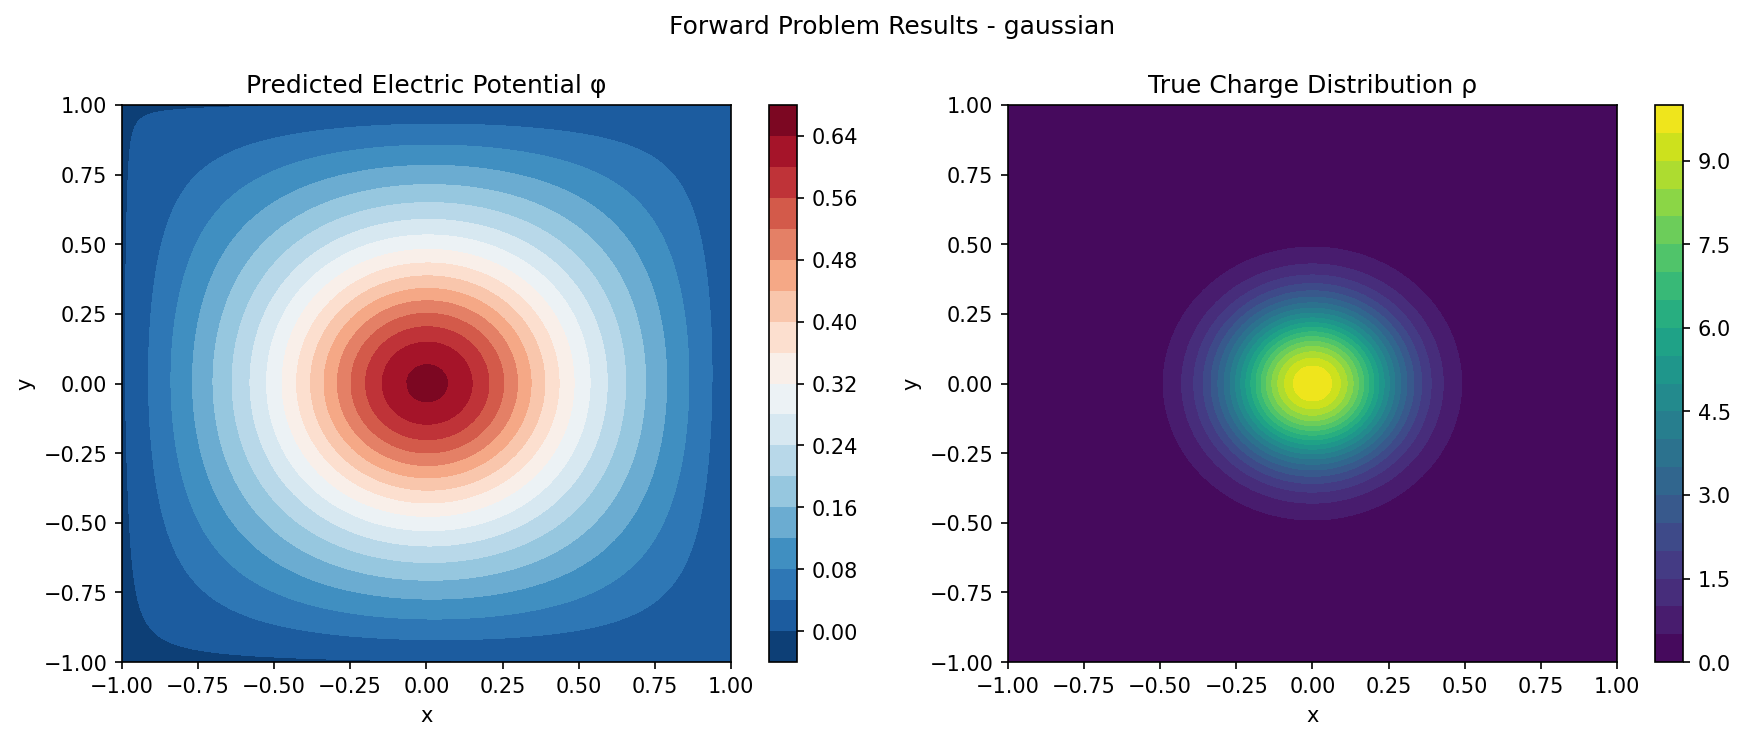
\includegraphics[width=0.9\textwidth]{figures/forward_gaussian_combined.png} \\
			\tiny 高斯电荷分布与对应电势场
		\end{column}
	\end{columns}
	\vspace{1em}
	\begin{block}{结论}
		PINN 能够准确求解给定电荷分布下的电势场。这些精确的电势场可用于生成逆问题的模拟测量数据。
	\end{block}
\end{frame}

%----------------------------------------------------------------------------------
\section{实验设置}
%----------------------------------------------------------------------------------
\begin{frame}
  \frametitle{实验设置}
  \begin{itemize}
    \item \textbf{计算域与边界:} 二维区域 $[-1, 1] \times [-1, 1]$,四边电势 $\phi = 0$。
    \item \textbf{电荷分布模型:}
        \begin{itemize}
            \item 方形电荷 (Square): 中心区域均匀分布,非光滑。
            \item 高斯电荷 (Gaussian): 中心高斯分布,光滑。
        \end{itemize}
    \item \textbf{神经网络结构:} 全连接网络,层大小: $[2, 64, 64, 64, 1]$ (正向) / $[2, 64, 64, 64, 2]$ (逆向),激活函数: $\tanh$。
    \item \textbf{训练参数:} AdamW 优化器,迭代次数 $12000$,学习率 $0.001$。
    \item \textbf{逆问题参数:}
        \begin{itemize}
            \item 数据点数量 (Measurement Points): $200, 400, 800, 1500$。
            \item 噪声水平 (Noise Levels): $0\%, 1\%, 2\%, 5\%$ (高斯噪声)。
        \end{itemize}
    \item \textbf{评估指标:} 相关系数 (Correlation Coefficient),辅以可视化结果。
  \end{itemize}
\end{frame}

%----------------------------------------------------------------------------------
\section{结果与分析}
%----------------------------------------------------------------------------------
\subsection{方形电荷重建}
\begin{frame}
  \frametitle{方形电荷逆向重建:相关系数}
  \begin{block}{相关系数 (Correlation Coefficient) - 方形电荷}
    \centering
    % 请在这里用 \begin{tabular}{...} ... \end{tabular} 插入你的表格
    \begin{tabular}{c|cccc}
        \toprule
         & 200点 & 400点 & 800点 & 1500点 \\
        \midrule
        0\%   & 0.864 & 0.879 & 0.872 & 0.868 \\
        1\%   & 0.858 & 0.860 & 0.871 & 0.869 \\
        2\%   & 0.840 & 0.845 & 0.866 & 0.875 \\
        5\%   & 0.815 & 0.795 & 0.855 & 0.837 \\
        \bottomrule
    \end{tabular}

    \small 方形电荷重建的相关系数普遍在0.8-0.88之间,难以完美恢复。
  \end{block}
\end{frame}
\begin{frame}
	\frametitle{方形电荷逆向重建:较优情况}
	\begin{center}
		\textbf{400点, 0\%噪声}\\
		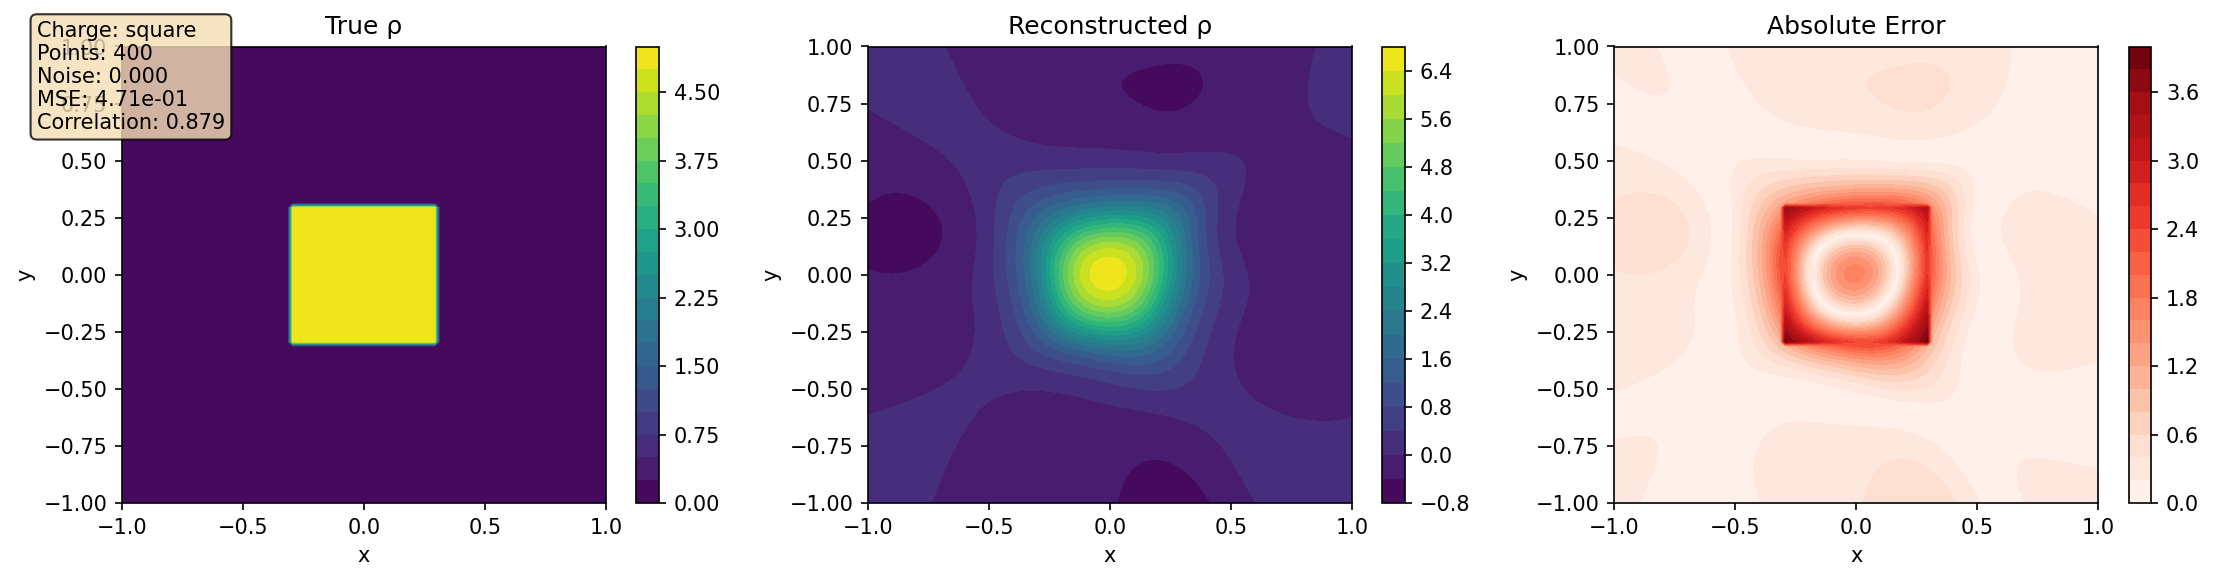
\includegraphics[width=0.95\textwidth]{figures/inverse_square_400pts_0noise_combined.png}
		% 上图应包含 rho_true, rho_estimated, error 三部分

		\small 相关系数: 0.879
	\end{center}
\end{frame}

\begin{frame}
	\frametitle{方形电荷逆向重建:中等情况}
	\begin{center}
		\textbf{400点, 1\%噪声}\\
		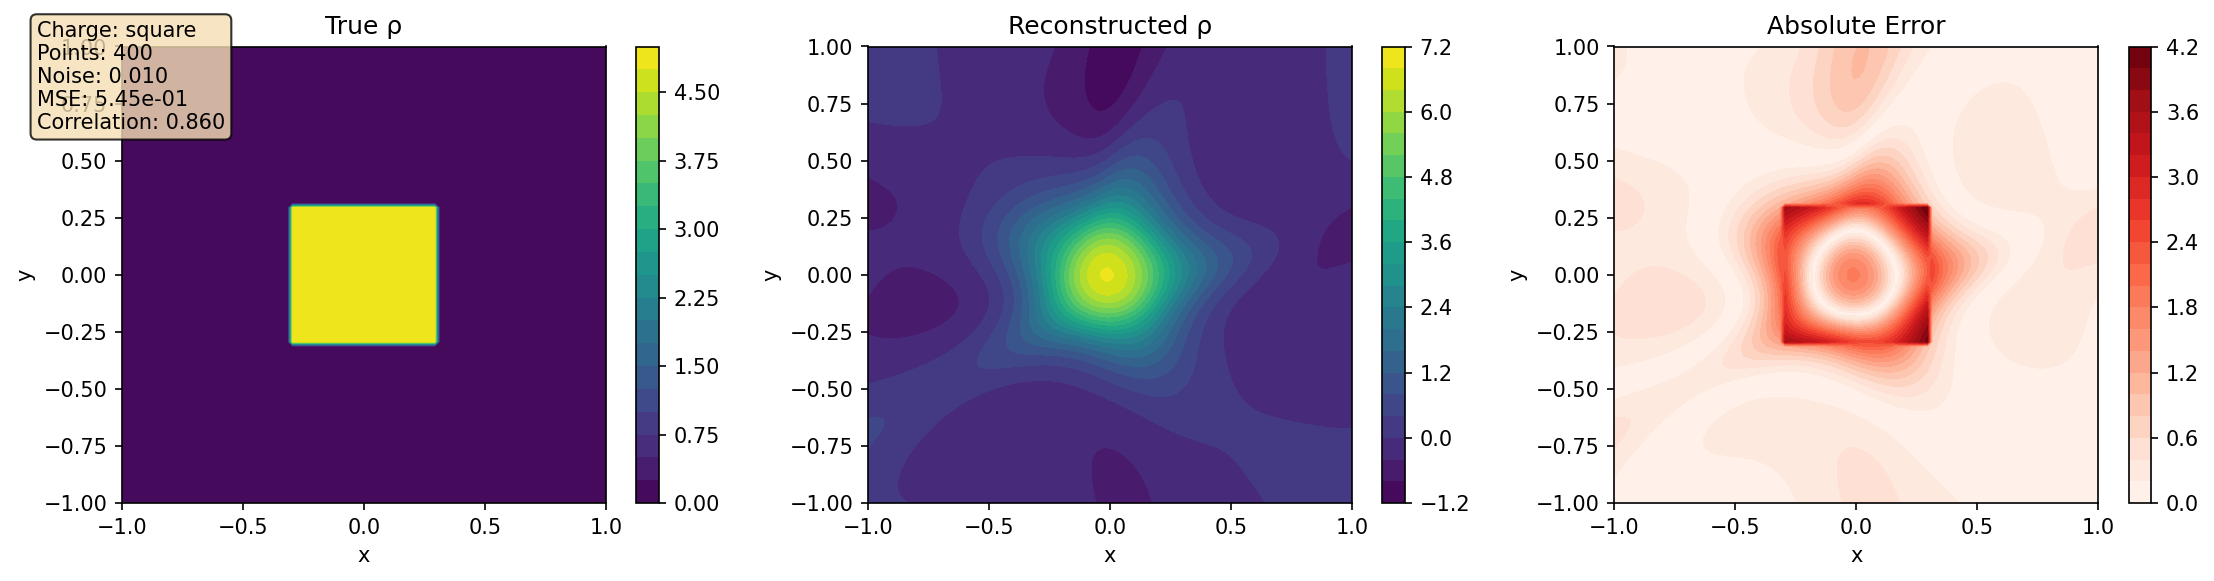
\includegraphics[width=0.95\textwidth]{figures/inverse_square_400pts_1noise_combined.png}
		% 上图应包含 rho_true, rho_estimated, error 三部分

		\small 相关系数: 0.860
	\end{center}
\end{frame}

\begin{frame}
	\frametitle{方形电荷逆向重建:较差情况}
	\begin{center}
		\textbf{400点, 5\%噪声}\\
		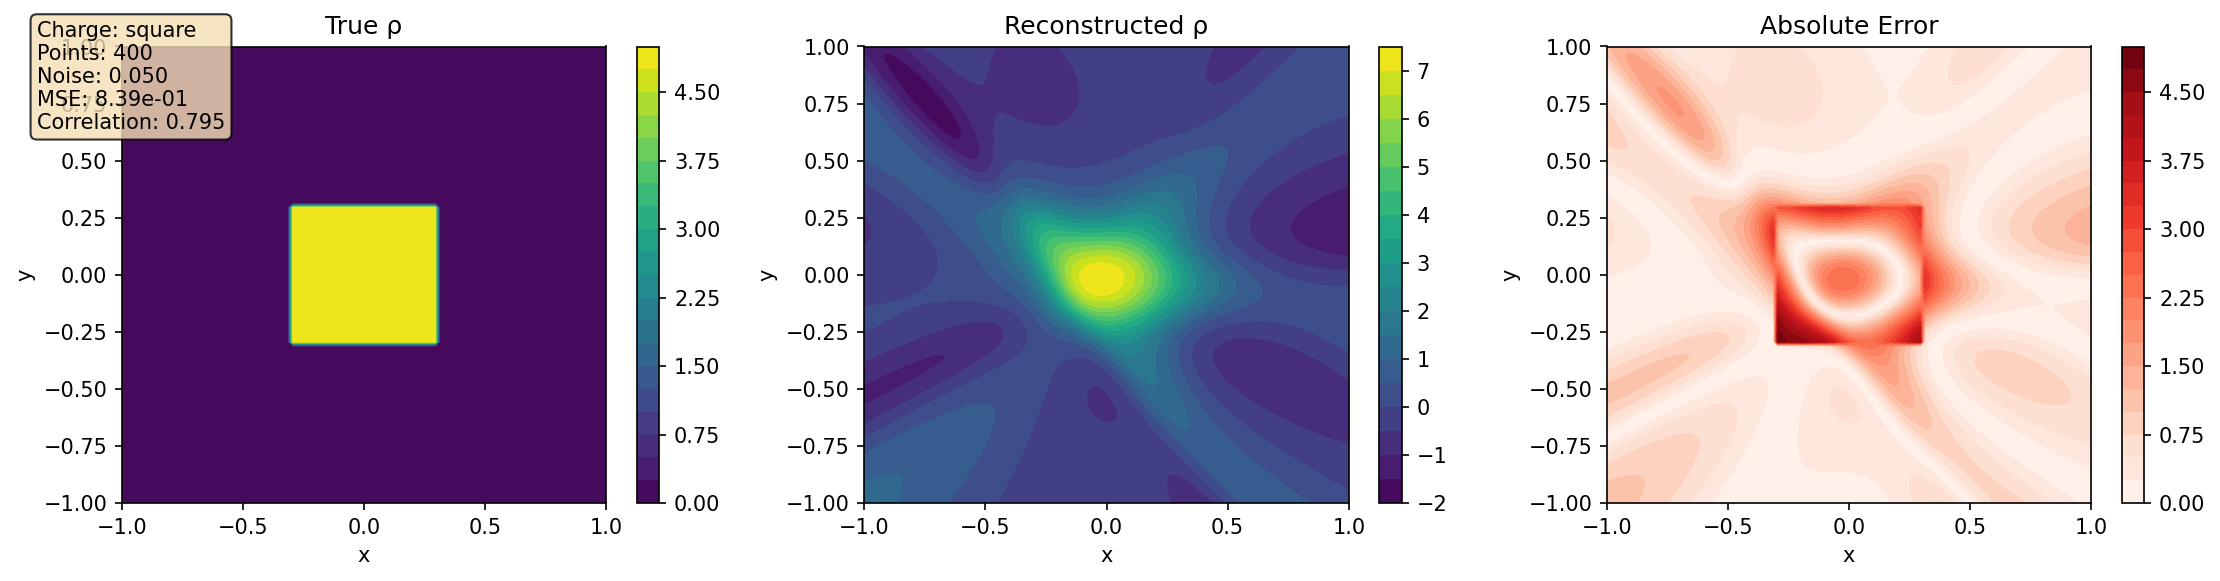
\includegraphics[width=0.95\textwidth]{figures/inverse_square_400pts_5noise_combined.png}
		% 上图应包含 rho_true, rho_estimated, error 三部分

		\small 相关系数: 0.795
	\end{center}
\end{frame}

\begin{frame}
	\frametitle{方形电荷重建分析}
	\begin{alertblock}{主要观察与分析}
		\begin{itemize}
				\item \textbf{形状失真:} 重建的电荷分布普遍失去方形的尖锐边缘,呈现为更平滑的类圆形。
				\item \textbf{数据点影响:} 增加数据点数量对相关系数的提升有限,对恢复边缘形状改善不明显。
				\item \textbf{噪声影响:} 噪声增加会进一步降低相关系数,使重建形状更弥散。
				\item \textbf{原因:} 神经网络的平滑性;高频信息(边缘)在重建和求二阶导数过程中易丢失。
		\end{itemize}
	\end{alertblock}
\end{frame}

\subsection{高斯电荷重建}
\begin{frame}
  \frametitle{高斯电荷逆向重建:相关系数}
  \begin{block}{相关系数 (Correlation Coefficient) - 高斯电荷}
    \centering
    \begin{tabular}{c|cccc}
        \toprule
        & 200点 & 400点 & 800点 & 1500点 \\
        \midrule
        0\%   & 0.985 & 0.982 & 0.981 & 0.987 \\
        1\%   & 0.977 & 0.984 & 0.985 & 0.983 \\
        2\%   & 0.940 & 0.975 & 0.978 & 0.983 \\
        5\%   & 0.747 & 0.862 & 0.961 & 0.952 \\
        \bottomrule
    \end{tabular}

    \small 高斯电荷重建的相关系数在数据质量较好时非常高,但受噪声和数据点影响。
  \end{block}
\end{frame}


\begin{frame}
	\frametitle{高斯电荷逆向重建:较优情况}
	\begin{center}
		\textbf{1500点, 0\%噪声}\\
		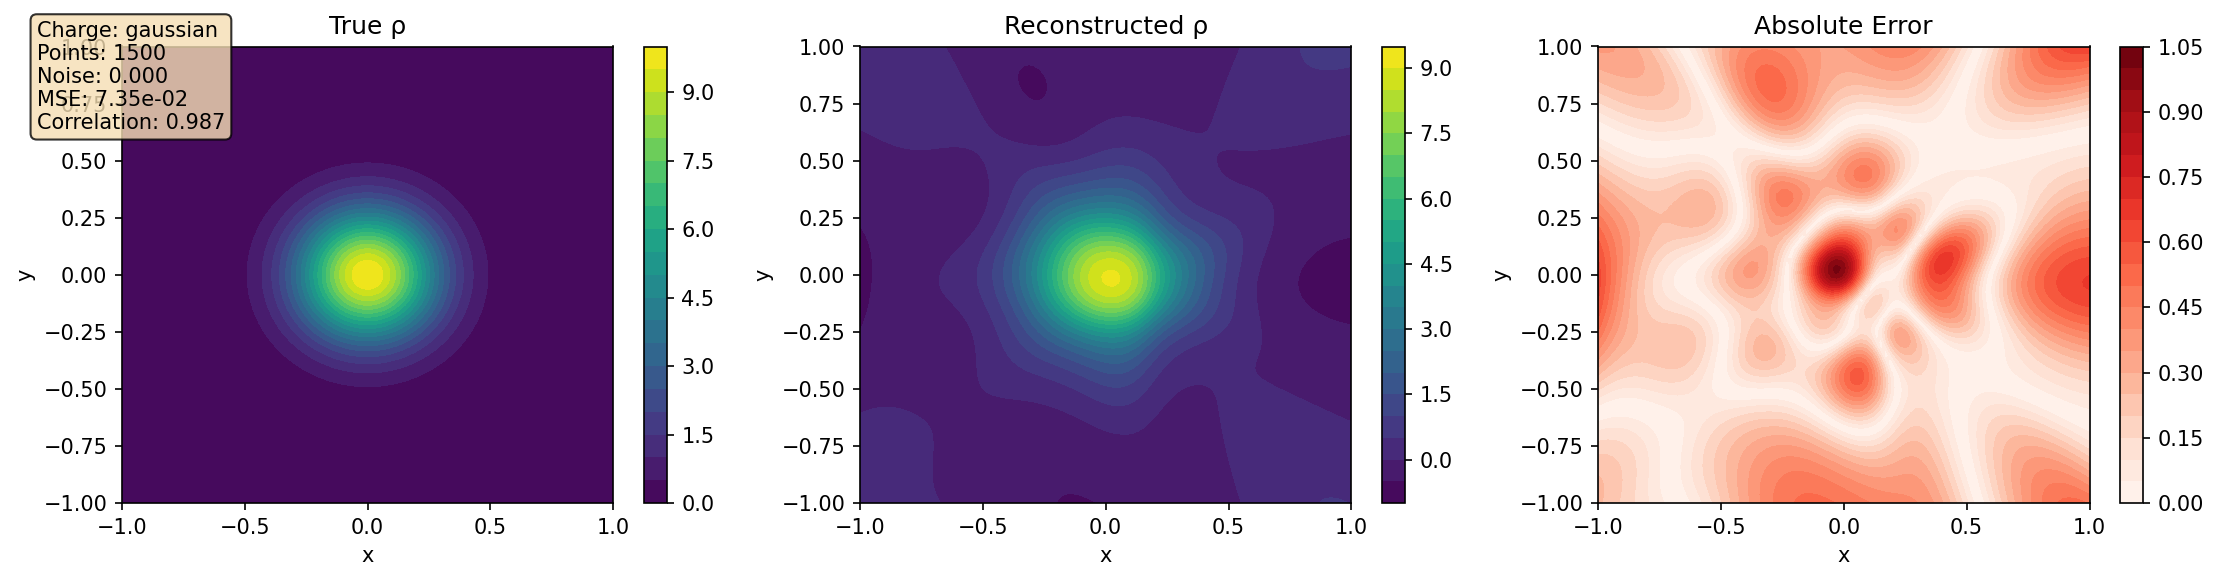
\includegraphics[width=0.95\textwidth]{figures/inverse_gaussian_1500pts_0noise_combined.png}
		% 上图应包含 rho_true, rho_estimated, error 三部分

		\small 相关系数: 0.987
	\end{center}
\end{frame}

\begin{frame}
	\frametitle{高斯电荷逆向重建:较差情况}
	\begin{center}
		\textbf{200点, 5\%噪声}\\
		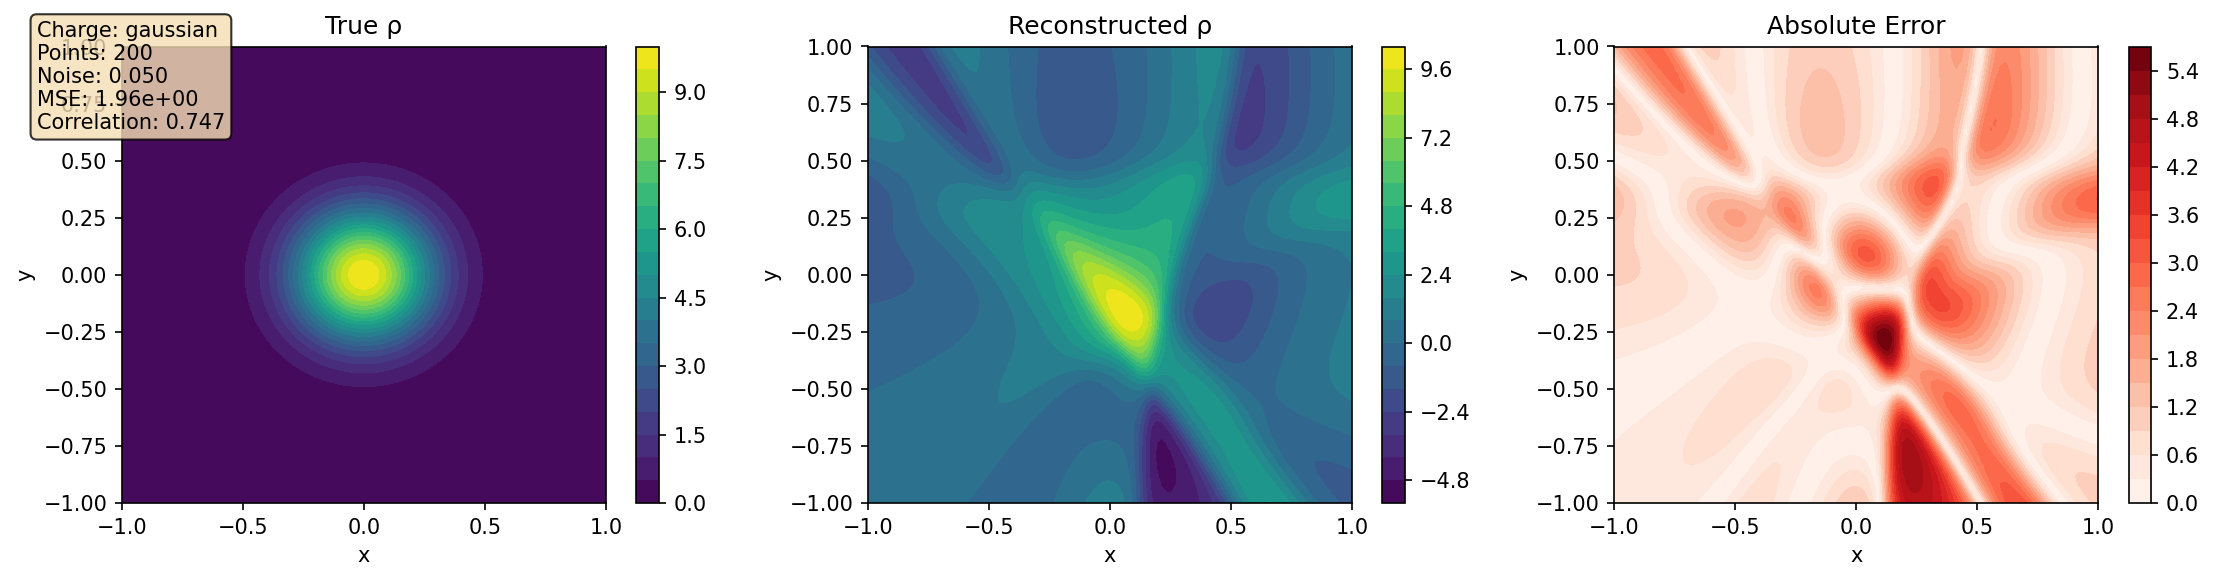
\includegraphics[width=0.95\textwidth]{figures/inverse_gaussian_200pts_5noise_combined.png}
		% 上图应包含 rho_true, rho_estimated, error 三部分

		\small 相关系数: 0.747
	\end{center}
\end{frame}

\begin{frame}
	\frametitle{高斯电荷重建分析}
	\begin{alertblock}{主要观察与分析}
		\begin{itemize}
			\item \textbf{形状匹配度高:} 在数据质量较好时,PINN能以高相关系数重建光滑的高斯分布。
			\item \textbf{数据点影响:} 增加数据点能显著提高重建的稳定性和准确性,尤其是在有噪声时。
			\item \textbf{噪声影响:} 噪声较大时,重建质量会显著下降,导致形状扭曲 (如 Corr=0.747 的情况)。
			\item \textbf{原因:} 光滑源与神经网络特性更匹配,但精确恢复仍需足量数据。
		\end{itemize}
	\end{alertblock}
\end{frame}

%----------------------------------------------------------------------------------
\section{总结与展望}
%----------------------------------------------------------------------------------
\begin{frame}
  \frametitle{总结}
  \begin{itemize}
    \item 本研究利用PINN成功实现了静电场正向计算和电荷分布的逆向重建。
    \pause
    \item \textbf{核心发现 1 (源光滑性):} PINN在重建光滑电荷分布(高斯)时表现优异,但在处理具有尖锐边缘的非光滑电荷分布(方形)时,难以完美恢复其形状,倾向于产生平滑近似。
    \pause
    \item \textbf{核心发现 2 (数据质量):} 重建精度显著依赖于测量数据的质量:
        \begin{itemize}
            \item \textbf{数据点数量:} 增加数据点对光滑源的改善更明显;对非光滑源的形状恢复改善有限。
            \item \textbf{噪声水平:} 噪声普遍降低重建质量,对光滑源的参数估计和非光滑源的形状稳定性均有影响。
        \end{itemize}
    \pause
    \item PINN为解决此类物理逆问题提供了一种有创新性的结合数据与物理约束的思路。
  \end{itemize}
\end{frame}

\begin{frame}
  \frametitle{展望}
    \begin{itemize}
        \item \textbf{改进非光滑源重建:}
            \begin{itemize}
                \item 探索具有更强高频特征表达能力的网络结构 (如傅里叶特征网络)。
                \item 研究特定的正则化方法 (如全变分正则化) 以鼓励分段常数解。
            \end{itemize}
        \item \textbf{优化采样策略:} 研究自适应采样或更优的固定采样策略,以提高数据效率。
        \item \textbf{扩展到更复杂问题:}
            \begin{itemize}
                \item 三维静电问题。
                \item 包含不同介质的静电问题。
                \item 其他物理场的逆问题。
            \end{itemize}
    \end{itemize}
\end{frame}

%--------------------
% 致谢
%--------------------
\begin{frame}
  \frametitle{致谢}
  \begin{itemize}
    \item 感谢孙悦淳学长提供的算力支持。
    \item 感谢各位老师和同学的聆听!
  \end{itemize}
  \vfill
  \centerline{\LARGE 谢谢!}
\end{frame}

\end{document}